\section{Introduction (Rough Draft)}

From a machine learning standpoint, Rock-Paper-Scissors is a simple classification problem. What we wanted to do was compare the accuracy of a trained neural network to that of a state-of-the-art computer vision algorithm. The difficulty here is that what we are analyzing (a hand) is the same object in different positions. This rules out algorithms such as colour histograms which use an object's colour for classification. One computer vision algorithm which has had much success in object recognition is Scale Invariant Feature Transform (SIFT) \cite{SIFT}. This algorithm uses keypoints -- defining features of an object -- to identify objects. SIFT does well at classifying objects even when they are rotated or scaled slightly. The neural network we used is a derivative of one that identified millions of objects from a thousand different categories with accuracies rivalling humans. We will compare these two approaches to object recognition to find out if a neural network is comparable to a state-of-the-art computer vision algorithm. We will be looking at both accuracy as well as how fast each method can run on a mid range computer. Ideally, these methods would be fast enough to run on a live video feed.

\subsection{Collecting Images}
Both methods need images of hands doing Rock, Paper, and Scissors to learn what each looks like. We began by imaging hands in these three positions. The hands were in various orientations (towards the camera, sideways, etc.) and the images were taken in different locations so there would be variations in background and lighting.  We also tried to account for different factors such as hand size, skin color, wrinkles, hair, etc. in order to cover as many cases as we can to get the best results. We captured 430 images in total with about 140 images for each of the three positions from numerous people using a simple laptop webcam. The neural network we decided to use required images which were 299$\times$299, so we cropped each of our images to this size. We then randomly split our images into a training set and a validation set with about the same number of images in each. This data was used by both the neural network and SIFT to ensure any differences in their performance were not a result of the data.

\begin{figure}[h]
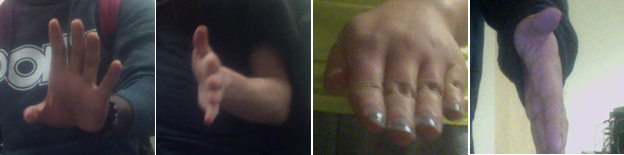
\includegraphics[scale=0.8]{paper_image_nn.png}
\centering
\caption{Training images of various paper hand gestures}
\end{figure}

\begin{figure}[h]
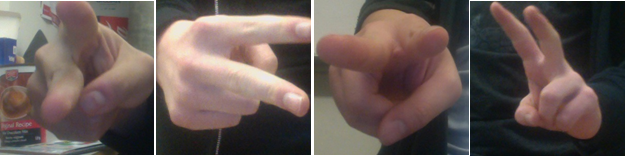
\includegraphics[scale=0.8]{scissors_image_nn.png}
\centering
\caption{Training images of various scissor hand gestures}
\end{figure}

\begin{figure}[h]
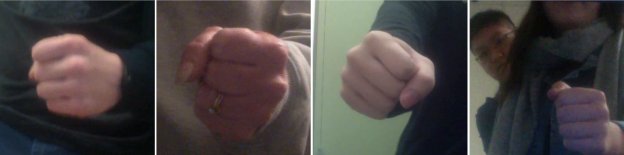
\includegraphics[scale=0.8]{rock_image_nn.png}
\centering
\caption{Training images of various rock hand gestures}
\end{figure}

\subsection{Hand Tracking}
Because we wanted to asses the possibility of these methods being used on a live video feed, we needed a method to crop the 1280$\times$720 images down to 299$\times$299 images containing as much of the hand as possible. This is basically hand tracking. To do this we used a computer vision algorithm called colour indexing \cite{swain}. This method uses a model of the object to be tracked and records the colour distribution of that model -- its colour histogram. Then, for each image to be analyzed, the likelihood of each of its pixel being part of the model is calculated using the model histogram. This produces a probability image. Finally, we use mean shift to find the most likely location of the hand. The benefit of this method is it's fast and can track a hand regardless of what position the hand is in. One drawback of this method is, since it's basically looking for skin colours, it can easily end up tracking the user's head instead of their hand. To address this, we decided that the camera should face the user's chest so their head is above the top of the view. This reduced the issue, however it still has trouble locating just the hand when the user also has their arm exposed. We used three images of just a hand as our models and were able to track a hand in realtime. 